% Created 2024-02-22 Thu 19:10
% Intended LaTeX compiler: pdflatex
\documentclass[11pt]{article}
\usepackage[utf8]{inputenc}
\usepackage[T1]{fontenc}
\usepackage{graphicx}
\usepackage{longtable}
\usepackage{wrapfig}
\usepackage{rotating}
\usepackage[normalem]{ulem}
\usepackage{amsmath}
\usepackage{amssymb}
\usepackage{capt-of}
\usepackage{hyperref}
\usepackage[margin=1in]{geometry}
\author{Malcolm Kahora, Vejay, Rohan, Tyler}
\date{\today}
\title{Homework 2\\\medskip
\large STA 307}
\hypersetup{
 pdfauthor={Malcolm Kahora, Vejay, Rohan, Tyler},
 pdftitle={Homework 2},
 pdfkeywords={},
 pdfsubject={},
 pdfcreator={Emacs 30.0.50 (Org mode 9.6.11)}, 
 pdflang={English}}

% Setup for code blocks [1/2]

\usepackage{fvextra}

\fvset{%
  commandchars=\\\{\},
  highlightcolor=white!95!black!80!blue,
  breaklines=true,
  breaksymbol=\color{white!60!black}\tiny\ensuremath{\hookrightarrow}}

% Make line numbers smaller and grey.
\renewcommand\theFancyVerbLine{\footnotesize\color{black!40!white}\arabic{FancyVerbLine}}

\usepackage{xcolor}

% In case engrave-faces-latex-gen-preamble has not been run.
\providecolor{EfD}{HTML}{f7f7f7}
\providecolor{EFD}{HTML}{28292e}

% Define a Code environment to prettily wrap the fontified code.
\usepackage[breakable,xparse]{tcolorbox}
\DeclareTColorBox[]{Code}{o}%
{colback=EfD!98!EFD, colframe=EfD!95!EFD,
  fontupper=\footnotesize\setlength{\fboxsep}{0pt},
  colupper=EFD,
  IfNoValueTF={#1}%
  {boxsep=2pt, arc=2.5pt, outer arc=2.5pt,
    boxrule=0.5pt, left=2pt}%
  {boxsep=2.5pt, arc=0pt, outer arc=0pt,
    boxrule=0pt, leftrule=1.5pt, left=0.5pt},
  right=2pt, top=1pt, bottom=0.5pt,
  breakable}

% Support listings with captions
\usepackage{float}
\floatstyle{plain}
\newfloat{listing}{htbp}{lst}
\newcommand{\listingsname}{Listing}
\floatname{listing}{\listingsname}
\newcommand{\listoflistingsname}{List of Listings}
\providecommand{\listoflistings}{\listof{listing}{\listoflistingsname}}


% Setup for code blocks [2/2]: syntax highlighting colors


\newcommand{\engravedthemedoomone}{%
\renewcommand\efstrut{\vrule height 2.1ex depth 0.8ex width 0pt}
\definecolor{EFD}{HTML}{bbc2cf}
\definecolor{EfD}{HTML}{282c34}
\renewcommand{\EFD}[1]{\textcolor{EFD}{##1}} % default
\definecolor{EFh}{HTML}{5B6268}
\renewcommand{\EFh}[1]{\textcolor{EFh}{##1}} % shadow
\definecolor{EFsc}{HTML}{98be65}
\renewcommand{\EFsc}[1]{\textcolor{EFsc}{##1}} % success
\definecolor{EFw}{HTML}{ECBE7B}
\renewcommand{\EFw}[1]{\textcolor{EFw}{##1}} % warning
\definecolor{EFe}{HTML}{ff6c6b}
\renewcommand{\EFe}[1]{\textcolor{EFe}{##1}} % error
\definecolor{EFc}{HTML}{5B6268}
\renewcommand{\EFc}[1]{\textcolor{EFc}{##1}} % font-lock-comment-face
\definecolor{EFcd}{HTML}{5B6268}
\renewcommand{\EFcd}[1]{\textcolor{EFcd}{##1}} % font-lock-comment-delimiter-face
\definecolor{EFs}{HTML}{98be65}
\renewcommand{\EFs}[1]{\textcolor{EFs}{##1}} % font-lock-string-face
\definecolor{EFd}{HTML}{83898d}
\renewcommand{\EFd}[1]{\textcolor{EFd}{##1}} % font-lock-doc-face
\definecolor{EFm}{HTML}{a9a1e1}
\renewcommand{\EFm}[1]{\textcolor{EFm}{##1}} % font-lock-doc-markup-face
\definecolor{EFk}{HTML}{51afef}
\renewcommand{\EFk}[1]{\textcolor{EFk}{##1}} % font-lock-keyword-face
\definecolor{EFb}{HTML}{c678dd}
\renewcommand{\EFb}[1]{\textcolor{EFb}{##1}} % font-lock-builtin-face
\definecolor{EFf}{HTML}{c678dd}
\renewcommand{\EFf}[1]{\textcolor{EFf}{##1}} % font-lock-function-name-face
\definecolor{EFv}{HTML}{dcaeea}
\renewcommand{\EFv}[1]{\textcolor{EFv}{##1}} % font-lock-variable-name-face
\definecolor{EFt}{HTML}{ECBE7B}
\renewcommand{\EFt}[1]{\textcolor{EFt}{##1}} % font-lock-type-face
\definecolor{EFo}{HTML}{a9a1e1}
\renewcommand{\EFo}[1]{\textcolor{EFo}{##1}} % font-lock-constant-face
\definecolor{EFwr}{HTML}{ECBE7B}
\renewcommand{\EFwr}[1]{\textcolor{EFwr}{##1}} % font-lock-warning-face
\definecolor{EFnc}{HTML}{51afef}
\renewcommand{\EFnc}[1]{\textcolor{EFnc}{\textbf{##1}}} % font-lock-negation-char-face
\definecolor{EFpp}{HTML}{51afef}
\renewcommand{\EFpp}[1]{\textcolor{EFpp}{\textbf{##1}}} % font-lock-preprocessor-face
\definecolor{EFrc}{HTML}{51afef}
\renewcommand{\EFrc}[1]{\textcolor{EFrc}{\textbf{##1}}} % font-lock-regexp-grouping-construct
\definecolor{EFrb}{HTML}{51afef}
\renewcommand{\EFrb}[1]{\textcolor{EFrb}{\textbf{##1}}} % font-lock-regexp-grouping-backslash
\definecolor{Efob}{HTML}{23272e}
\renewcommand{\EFob}[1]{\colorbox{Efob}{\efstrut{}##1}} % org-block
\renewcommand{\EFhn}[1]{##1} % highlight-numbers-number
\renewcommand{\EFhq}[1]{##1} % highlight-quoted-quote
\renewcommand{\EFhs}[1]{##1} % highlight-quoted-symbol
\definecolor{EFrda}{HTML}{51afef}
\renewcommand{\EFrda}[1]{\textcolor{EFrda}{##1}} % rainbow-delimiters-depth-1-face
\definecolor{EFrdb}{HTML}{c678dd}
\renewcommand{\EFrdb}[1]{\textcolor{EFrdb}{##1}} % rainbow-delimiters-depth-2-face
\definecolor{EFrdc}{HTML}{98be65}
\renewcommand{\EFrdc}[1]{\textcolor{EFrdc}{##1}} % rainbow-delimiters-depth-3-face
\definecolor{EFrdd}{HTML}{a9a1e1}
\renewcommand{\EFrdd}[1]{\textcolor{EFrdd}{##1}} % rainbow-delimiters-depth-4-face
\definecolor{EFrde}{HTML}{4db5bd}
\renewcommand{\EFrde}[1]{\textcolor{EFrde}{##1}} % rainbow-delimiters-depth-5-face
\definecolor{EFrdf}{HTML}{51afef}
\renewcommand{\EFrdf}[1]{\textcolor{EFrdf}{##1}} % rainbow-delimiters-depth-6-face
\definecolor{EFrdg}{HTML}{c678dd}
\renewcommand{\EFrdg}[1]{\textcolor{EFrdg}{##1}} % rainbow-delimiters-depth-7-face
\definecolor{EFrdh}{HTML}{98be65}
\renewcommand{\EFrdh}[1]{\textcolor{EFrdh}{##1}} % rainbow-delimiters-depth-8-face
\definecolor{EFrdi}{HTML}{a9a1e1}
\renewcommand{\EFrdi}[1]{\textcolor{EFrdi}{##1}} % rainbow-delimiters-depth-9-face
}

\newcommand\efstrut{\vrule height 2.1ex depth 0.8ex width 0pt}
\definecolor{EFD}{HTML}{EEFFFF}
\definecolor{EfD}{HTML}{292D3E}
\newcommand{\EFD}[1]{\textcolor{EFD}{#1}} % default
\definecolor{EFh}{HTML}{676E95}
\newcommand{\EFh}[1]{\textcolor{EFh}{#1}} % shadow
\definecolor{EFsc}{HTML}{c3e88d}
\newcommand{\EFsc}[1]{\textcolor{EFsc}{#1}} % success
\definecolor{EFw}{HTML}{ffcb6b}
\newcommand{\EFw}[1]{\textcolor{EFw}{#1}} % warning
\definecolor{EFe}{HTML}{ff5370}
\newcommand{\EFe}[1]{\textcolor{EFe}{#1}} % error
\definecolor{EFc}{HTML}{676E95}
\newcommand{\EFc}[1]{\textcolor{EFc}{#1}} % font-lock-comment-face
\definecolor{EFcd}{HTML}{676E95}
\newcommand{\EFcd}[1]{\textcolor{EFcd}{#1}} % font-lock-comment-delimiter-face
\definecolor{EFs}{HTML}{c3e88d}
\newcommand{\EFs}[1]{\textcolor{EFs}{#1}} % font-lock-string-face
\definecolor{EFd}{HTML}{8d92af}
\newcommand{\EFd}[1]{\textcolor{EFd}{#1}} % font-lock-doc-face
\definecolor{EFm}{HTML}{f78c6c}
\newcommand{\EFm}[1]{\textcolor{EFm}{#1}} % font-lock-doc-markup-face
\definecolor{EFk}{HTML}{89DDFF}
\newcommand{\EFk}[1]{\textcolor{EFk}{#1}} % font-lock-keyword-face
\definecolor{EFb}{HTML}{82aaff}
\newcommand{\EFb}[1]{\textcolor{EFb}{#1}} % font-lock-builtin-face
\definecolor{EFf}{HTML}{82aaff}
\newcommand{\EFf}[1]{\textcolor{EFf}{#1}} % font-lock-function-name-face
\definecolor{EFv}{HTML}{ffcb6b}
\newcommand{\EFv}[1]{\textcolor{EFv}{#1}} % font-lock-variable-name-face
\definecolor{EFt}{HTML}{c792ea}
\newcommand{\EFt}[1]{\textcolor{EFt}{#1}} % font-lock-type-face
\definecolor{EFo}{HTML}{f78c6c}
\newcommand{\EFo}[1]{\textcolor{EFo}{#1}} % font-lock-constant-face
\definecolor{EFwr}{HTML}{ffcb6b}
\newcommand{\EFwr}[1]{\textcolor{EFwr}{#1}} % font-lock-warning-face
\definecolor{EFnc}{HTML}{89DDFF}
\newcommand{\EFnc}[1]{\textcolor{EFnc}{\textbf{#1}}} % font-lock-negation-char-face
\definecolor{EFpp}{HTML}{89DDFF}
\newcommand{\EFpp}[1]{\textcolor{EFpp}{\textbf{#1}}} % font-lock-preprocessor-face
\definecolor{EFrc}{HTML}{89DDFF}
\newcommand{\EFrc}[1]{\textcolor{EFrc}{\textbf{#1}}} % font-lock-regexp-grouping-construct
\definecolor{EFrb}{HTML}{89DDFF}
\newcommand{\EFrb}[1]{\textcolor{EFrb}{\textbf{#1}}} % font-lock-regexp-grouping-backslash
\definecolor{Efob}{HTML}{232635}
\newcommand{\EFob}[1]{\colorbox{Efob}{\efstrut{}#1}} % org-block
\newcommand{\EFhn}[1]{#1} % highlight-numbers-number
\newcommand{\EFhq}[1]{#1} % highlight-quoted-quote
\newcommand{\EFhs}[1]{#1} % highlight-quoted-symbol
\definecolor{EFrda}{HTML}{c792ea}
\newcommand{\EFrda}[1]{\textcolor{EFrda}{#1}} % rainbow-delimiters-depth-1-face
\definecolor{EFrdb}{HTML}{f78c6c}
\newcommand{\EFrdb}[1]{\textcolor{EFrdb}{#1}} % rainbow-delimiters-depth-2-face
\definecolor{EFrdc}{HTML}{c3e88d}
\newcommand{\EFrdc}[1]{\textcolor{EFrdc}{#1}} % rainbow-delimiters-depth-3-face
\definecolor{EFrdd}{HTML}{89DDFF}
\newcommand{\EFrdd}[1]{\textcolor{EFrdd}{#1}} % rainbow-delimiters-depth-4-face
\definecolor{EFrde}{HTML}{bb80b3}
\newcommand{\EFrde}[1]{\textcolor{EFrde}{#1}} % rainbow-delimiters-depth-5-face
\definecolor{EFrdf}{HTML}{ffcb6b}
\newcommand{\EFrdf}[1]{\textcolor{EFrdf}{#1}} % rainbow-delimiters-depth-6-face
\definecolor{EFrdg}{HTML}{82aaff}
\newcommand{\EFrdg}[1]{\textcolor{EFrdg}{#1}} % rainbow-delimiters-depth-7-face
\definecolor{EFrdh}{HTML}{44b9b1}
\newcommand{\EFrdh}[1]{\textcolor{EFrdh}{#1}} % rainbow-delimiters-depth-8-face
\definecolor{EFrdi}{HTML}{80cbc4}
\newcommand{\EFrdi}[1]{\textcolor{EFrdi}{#1}} % rainbow-delimiters-depth-9-face
\begin{document}

\maketitle
{\engravedthemedoomone\begin{Code}
\begin{Verbatim}
\color{EFD}
\EFk{import} numpy \EFk{as} np
\EFk{import} pandas \EFk{as} pd
\EFk{import} matplotlib.pyplot \EFk{as} plt
\EFk{from} ISLP \EFk{import} load\_data
\EFk{from} sklearn.datasets \EFk{import} load\_iris
\EFk{from} sklearn.preprocessing \EFk{import} StandardScaler
\EFk{from} sklearn.decomposition \EFk{import} PCA

\EFv{AUTO} = load\_data\EFrda{(}\EFs{"Auto"}\EFrda{)}
\end{Verbatim}
\end{Code}}

\section*{Question 1}
\label{sec:orge6ad14b}


\begin{Code}
\begin{Verbatim}
\color{EFD}
\EFv{selected\_coloumns} = \EFrda{[}\EFs{'mpg'},\EFs{'cylinders'}, \EFs{'displacement'},  \EFs{'weight'}, \EFs{'acceleration'}, \EFrda{]}
\EFv{X} = AUTO\EFrda{[}selected\_coloumns\EFrda{]}
\EFv{y} = AUTO\EFrda{[}\EFs{'origin'}\EFrda{]} \EFcd{\# }\EFc{Origin of car (1. American, 2. European, 3. Japanese)}
\EFb{print}\EFrda{(}X.head\EFrda{)}

\EFb{print}\EFrda{(}\EFs{"American cars: \{0\}"}.\EFb{format}\EFrdb{(}\EFrdc{(}y == 1\EFrdc{)}.\EFb{sum}\EFrdc{(}\EFrdc{)}\EFrdb{)}\EFrda{)} \EFcd{\# }\EFc{American}
\EFb{print}\EFrda{(}\EFs{"European cars: \{0\}"}.\EFb{format}\EFrdb{(}\EFrdc{(}y == 2\EFrdc{)}.\EFb{sum}\EFrdc{(}\EFrdc{)}\EFrdb{)}\EFrda{)} \EFcd{\# }\EFc{European}
\EFb{print}\EFrda{(}\EFs{"Japanese cars: \{0\}"}.\EFb{format}\EFrdb{(}\EFrdc{(}y == 3\EFrdc{)}.\EFb{sum}\EFrdc{(}\EFrdc{)}\EFrdb{)}\EFrda{)} \EFcd{\# }\EFc{Japanese}
\end{Verbatim}
\end{Code}

\begin{verbatim}
<bound method NDFrame.head of       mpg  cylinders  displacement  weight  acceleration
0    18.0          8         307.0    3504          12.0
1    15.0          8         350.0    3693          11.5
2    18.0          8         318.0    3436          11.0
3    16.0          8         304.0    3433          12.0
4    17.0          8         302.0    3449          10.5
..    ...        ...           ...     ...           ...
387  27.0          4         140.0    2790          15.6
388  44.0          4          97.0    2130          24.6
389  32.0          4         135.0    2295          11.6
390  28.0          4         120.0    2625          18.6
391  31.0          4         119.0    2720          19.4

[392 rows x 5 columns]>
American cars: 245
European cars: 68
Japanese cars: 79
\end{verbatim}

\section*{Question 2}
\label{sec:orgf54ac04}



\begin{Code}
\begin{Verbatim}
\color{EFD}\EFb{print}\EFrda{(}\EFs{"Standard deviation"}\EFrda{)}
\EFb{print}\EFrda{(}X.std\EFrdb{(}\EFrdb{)}\EFrda{)}
\EFb{print}\EFrda{(}\EFs{"}\EFo{\char92{}n}\EFs{"}\EFrda{)}
\EFb{print}\EFrda{(}\EFs{"Mean"}\EFrda{)}
\EFb{print}\EFrda{(}X.mean\EFrdb{(}\EFrdb{)}\EFrda{)}
\end{Verbatim}
\end{Code}

\begin{verbatim}
Standard deviation
mpg               7.805007
cylinders         1.705783
displacement    104.644004
weight          849.402560
acceleration      2.758864
dtype: float64


Mean
mpg               23.445918
cylinders          5.471939
displacement     194.411990
weight          2977.584184
acceleration      15.541327
dtype: float64
\end{verbatim}

\section*{Qustion 3}
\label{sec:org5f38fec}

\begin{Code}
\begin{Verbatim}
\color{EFD}
\EFv{scaler} = StandardScaler\EFrda{(}\EFrda{)}
scaler.fit\EFrda{(}X\EFrda{)}
\EFv{X\_standardized} = scaler.transform\EFrda{(}X\EFrda{)}

\EFb{print}\EFrda{(}\EFs{"Means: "},np.mean\EFrdb{(}X\_standardized,axis=0\EFrdb{)}\EFrda{)}
\EFb{print}\EFrda{(}\EFs{"Standard deviations: "},np.std\EFrdb{(}X\_standardized,axis=0\EFrdb{)}\EFrda{)}

\EFb{print}\EFrda{(}\EFs{"Original data size:"},X.shape\EFrda{)}
\EFcd{\# }\EFc{Implement PCA with 2 principal components}
\EFv{pca} = PCA\EFrda{(}n\_components=2\EFrda{)}

\EFcd{\# }\EFc{Fit the PCA model to the data and transform the data}
\EFv{X\_reduced} = pca.fit\_transform\EFrda{(}X\_standardized\EFrda{)}
\EFb{print}\EFrda{(}\EFs{"Reduced data size:"}, X\_reduced.shape\EFrda{)}

\EFcd{\#}\EFc{principal components}
\EFv{components} = pca.components\_
\EFv{x} = np.arange\EFrda{(}components.shape\EFrdb{[}1\EFrdb{]}\EFrda{)} \EFcd{\# }\EFc{6}

\EFcd{\# }\EFc{Plot the first and second principal components}
plt.plot\EFrda{(}x, components\EFrdb{[}0\EFrdb{]}, label=\EFs{'φ1'}\EFrda{)}
plt.plot\EFrda{(}x, components\EFrdb{[}1\EFrdb{]}, label=\EFs{'φ2'}\EFrda{)}

\EFcd{\# }\EFc{Define feature names as tick labels}
\EFv{names} = \EFrda{[}\EFs{'mpg'}, \EFs{'cylinders'}, \EFs{'displacement'}, \EFs{'weight'}, \EFs{'acceleration'}\EFrda{]}
plt.xticks\EFrda{(}ticks=x, labels=selected\_coloumns, rotation=45\EFrda{)}

\EFcd{\# }\EFc{Labeling the axes and the legend}
plt.xlabel\EFrda{(}\EFs{'Features'}\EFrda{)}
plt.ylabel\EFrda{(}\EFs{'Principal Component Weights'}\EFrda{)}
plt.title\EFrda{(}\EFs{'Principal Component Weights per Feature'}\EFrda{)}
plt.legend\EFrda{(}\EFrda{)}

\EFcd{\# }\EFc{Show plot}
plt.tight\_layout\EFrda{(}\EFrda{)}
plt.savefig\EFrda{(}\EFs{"plot.png"}, bbox\_inches=\EFs{'tight'}\EFrda{)}
\EFcd{\# }\EFc{plt.show()}
\end{Verbatim}
\end{Code}

\begin{center}
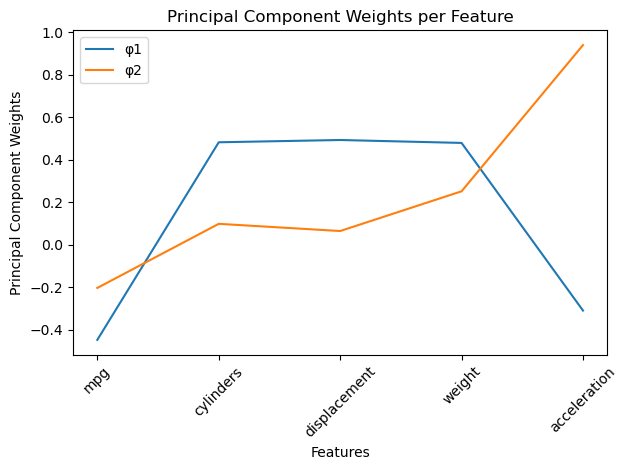
\includegraphics[width=.9\linewidth]{plot.png}
\end{center}
\end{document}
